\documentclass[aspectratio=169,11pt]{beamer}

\usepackage{fontspec}
\usepackage{polyglossia}
\setdefaultlanguage{russian}
\setotherlanguage{english}
\usepackage{unicode-math}
\usepackage{tikz}
\usetikzlibrary{arrows.meta,positioning,calc}
\usepackage{booktabs}
\usepackage{graphicx}
\usepackage{xcolor}

\setsansfont{Liberation Sans}[Ligatures=TeX]
\setmonofont{Liberation Mono}[Scale=0.9]
\setmathfont{texgyrepagella-math.otf}
\usefonttheme{professionalfonts}

\definecolor{navy}{HTML}{0B2545}
\definecolor{deep}{HTML}{13315C}
\definecolor{sun}{HTML}{E8871E}
\definecolor{teal}{HTML}{2A9D8F}
\definecolor{muted}{HTML}{5C677D}
\definecolor{paper}{HTML}{F4F6F8}
\definecolor{pale}{HTML}{E3E9F0}
\definecolor{edge}{HTML}{CBD5E0}
\definecolor{lighttext}{HTML}{C9D3E0}

\setbeamercolor{normal text}{fg=navy,bg=white}
\setbeamercolor{structure}{fg=navy}
\setbeamercolor{frametitle}{fg=navy,bg=white}
\setbeamercolor{alerted text}{fg=sun}
\setbeamercolor{footrule}{bg=sun}
\setbeamercolor{foottext}{bg=white,fg=muted}
\setbeamercolor{boxbg}{bg=paper,fg=navy}
\setbeamercolor{caption name}{fg=muted}

\setbeamertemplate{navigation symbols}{}
\setbeamersize{text margin left=7mm,text margin right=7mm}

\setbeamerfont{frametitle}{size=\Large,series=\bfseries}
\setbeamerfont{framesubtitle}{size=\small,series=\mdseries}

\setbeamertemplate{frametitle}{%
  \nointerlineskip
  \begin{beamercolorbox}[wd=\paperwidth,sep=0pt,leftskip=7mm,rightskip=7mm]{frametitle}%
    \vskip3.0mm
    \usebeamerfont{frametitle}\insertframetitle\par
    \vskip1.5mm
    {\color{sun}\rule{16mm}{1.6pt}}%
    \vskip1.5mm
  \end{beamercolorbox}%
}

\setbeamertemplate{footline}{%
  \begin{beamercolorbox}[wd=\paperwidth,ht=0.6pt,dp=0pt]{footrule}\end{beamercolorbox}%
  \hbox{%
    \begin{beamercolorbox}[wd=.5\paperwidth,ht=2.5ex,dp=1.1ex,leftskip=7mm]{foottext}%
      {\scriptsize ИСЗФ СО РАН}%
    \end{beamercolorbox}%
    \begin{beamercolorbox}[wd=.5\paperwidth,ht=2.5ex,dp=1.1ex,rightskip=7mm,right]{foottext}%
      {\scriptsize\insertframenumber\,/\,24}%
    \end{beamercolorbox}}%
}

\setbeamertemplate{itemize item}{\raisebox{0.12ex}{\scriptsize\textcolor{sun}{\textbullet}}}
\setbeamertemplate{itemize subitem}{\raisebox{0.12ex}{\scriptsize\textcolor{teal}{--}}}
\setbeamertemplate{enumerate item}{\textcolor{sun}{\bfseries\insertenumlabel.}}

\tikzset{
  card/.style={draw=edge,fill=paper,rounded corners=2.5pt,align=left,inner sep=3.2mm},
  chip/.style={draw=edge,fill=paper,rounded corners=1.5pt,align=center,
    inner sep=1.6mm,text=navy,font=\scriptsize},
  arr/.style={-{Stealth[length=2.2mm,width=1.8mm]},draw=muted,line width=0.9pt},
}

\newcommand{\source}[1]{\par\vspace{1.4mm}{\scriptsize\color{muted}#1}}
\newcommand{\bigresult}[1]{{\fontsize{27}{31}\selectfont\bfseries\color{sun}#1}}
\newcommand{\key}[1]{{\color{deep}\bfseries#1}}
\newcommand{\fig}[2][]{\includegraphics[#1]{figures/#2}}

\begin{document}

% ---------------------------------------------------------------- 1
{\setbeamertemplate{background canvas}{%
  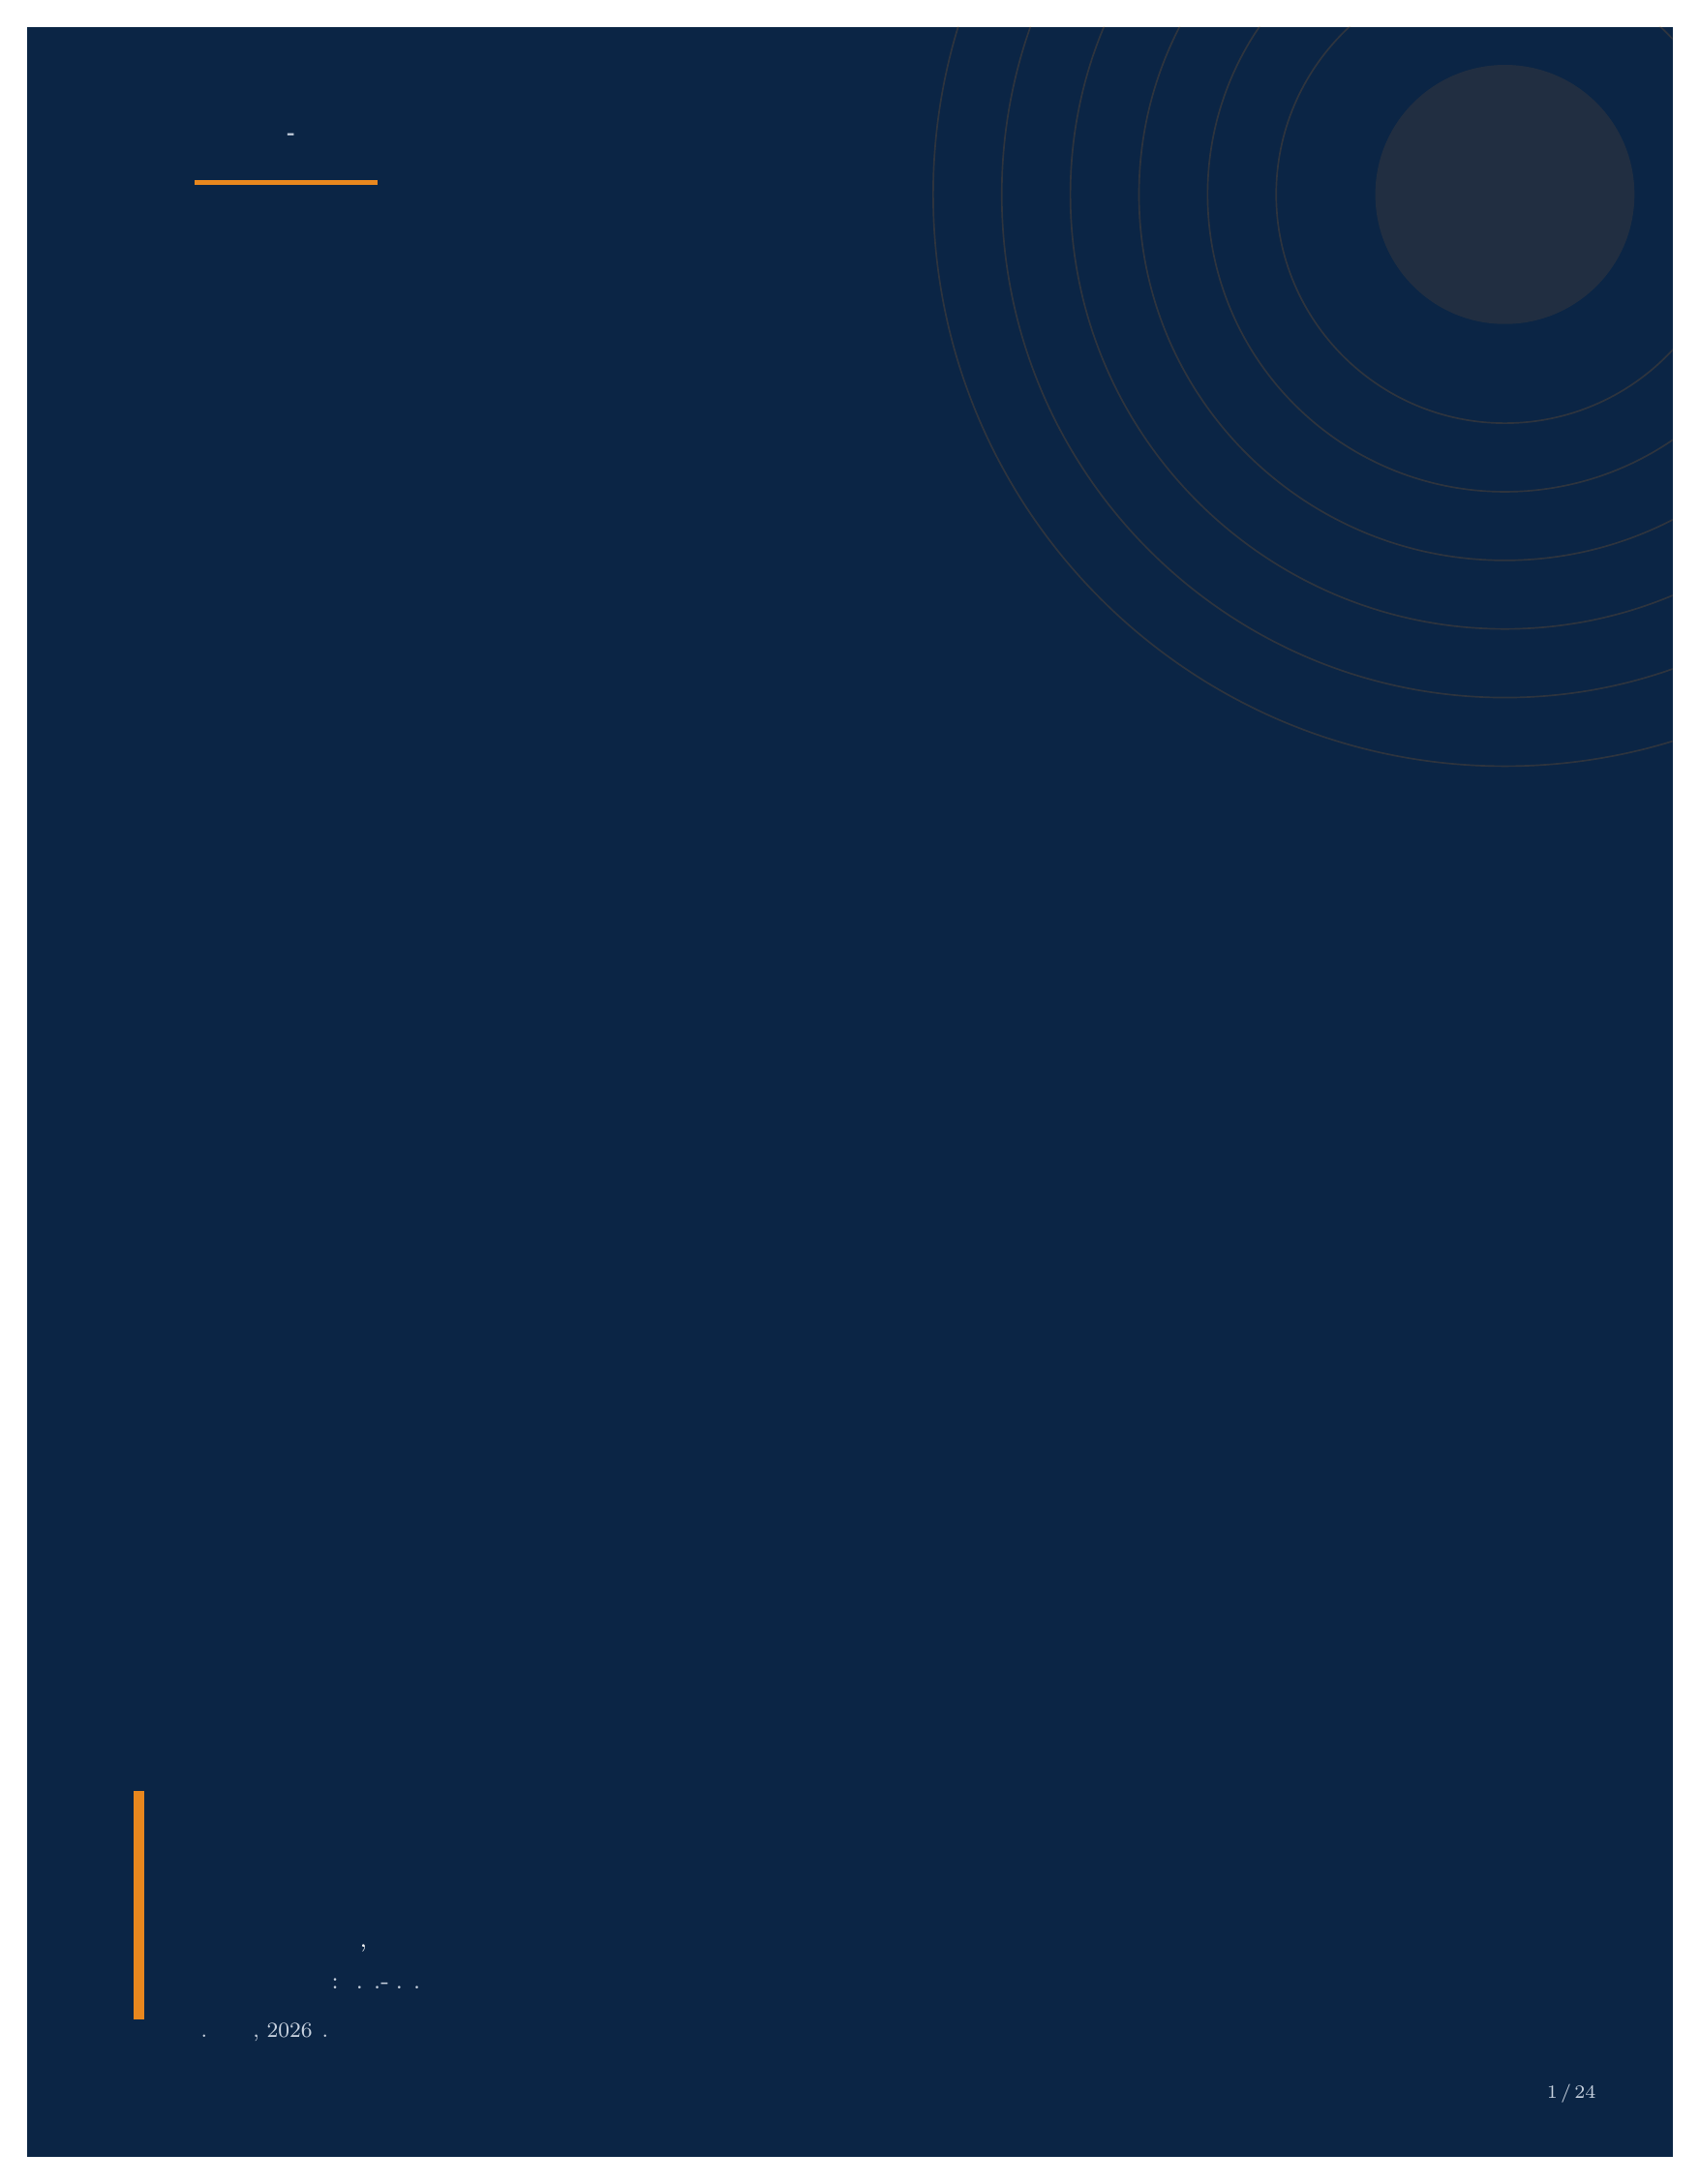
\begin{tikzpicture}[x=1cm,y=1cm]
    \useasboundingbox (0,0) rectangle (\paperwidth,\paperheight);
    \fill[navy] (0,0) rectangle (\paperwidth,\paperheight);
    \begin{scope}
      \clip (0,0) rectangle (\paperwidth,\paperheight);
      \foreach \r in {3.0,3.9,4.8,5.7,6.6,7.5} {
        \draw[sun,opacity=0.16,line width=0.6pt]
          ($(\paperwidth,\paperheight)+(-2.2,-2.2)$) circle[radius=\r];
      }
      \fill[sun,opacity=0.10]
        ($(\paperwidth,\paperheight)+(-2.2,-2.2)$) circle[radius=1.7];
    \end{scope}
    \fill[sun] (1.4,1.8) rectangle ++(0.14,3.0);

    \node[anchor=north west,inner sep=0]
      at (2.2,\paperheight-1.4cm) {%
        {\scriptsize\color{lighttext}\bfseries
          ИНСТИТУТ СОЛНЕЧНО-ЗЕМНОЙ ФИЗИКИ СО РАН}};
    \node[anchor=north west,inner sep=0]
      at (2.2,\paperheight-2.0cm) {%
        {\color{sun}\rule{24mm}{1.8pt}}};
    \node[anchor=north west,inner sep=0,align=left,text=white,text width=134mm]
      at (2.2,\paperheight-2.6cm) {%
        {\fontsize{21}{26}\selectfont\bfseries
          Взаимосвязь солнечного ветра\\[1mm]
          и характеристик ионосферы Земли}};
    \node[anchor=north west,inner sep=0,align=left]
      at (2.2,\paperheight-5.2cm) {%
        {\normalsize\color{lighttext}
          }};

    \node[anchor=south west,inner sep=0,align=left,text=white]
      at (2.2,1.5) {%
        \begin{minipage}{134mm}
          {\small Салимов Борис Гудратович, научный сотрудник}\\[1.2mm]
          {\small\color{lighttext}Научный руководитель: д.\,ф.-м.\,н.
            Ясюкевич Юрий Владимирович}\\[2.2mm]
          {\footnotesize\color{lighttext}г.\,Иркутск, 2026\,г.}
        \end{minipage}};

    \node[anchor=south east,inner sep=0,font=\scriptsize,text=lighttext]
      at (\paperwidth-1.0cm,0.7) {1\,/\,24};
  \end{tikzpicture}}
\begin{frame}[plain]\vspace*{0pt}\end{frame}}

% ---------------------------------------------------------------- 2
\begin{frame}[t]{План}
\vspace{1mm}
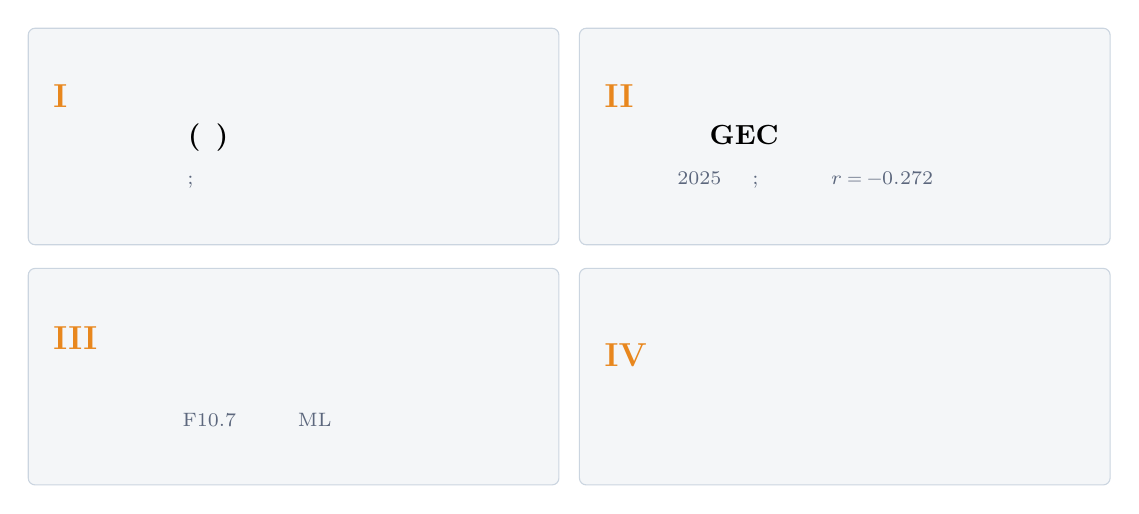
\begin{tikzpicture}[x=1cm,y=1cm]
  \node[card,anchor=north west,text width=6.1cm,minimum height=2.75cm] (c1) at (0,0) {%
    {\color{sun}\bfseries\large I}\\[0.4mm]
    {\bfseries Корональные дыры (КД)}\\[0.9mm]
    {\scriptsize\color{muted}Сибирский радиогелиограф; регистрирация КД}};
  \node[card,anchor=north west,text width=6.1cm,minimum height=2.75cm] (c2) at (7.0,0) {%
    {\color{sun}\bfseries\large II}\\[0.4mm]
    {\bfseries Площадь КД и GEC}\\[0.9mm]
    {\scriptsize\color{muted}Годовой ряд 2025 года; корреляция $r=-0.272$}};
  \node[card,anchor=north west,text width=6.1cm,minimum height=2.75cm] (c3) at (0,-3.05) {%
    {\color{sun}\bfseries\large III}\\[0.4mm]
    {\bfseries Прогноз ПЭС}\\[0.9mm]
    {\scriptsize\color{muted}Карты ПЭС по индексу F10.7 методами ML}};
  \node[card,anchor=north west,text width=6.1cm,minimum height=2.75cm] (c4) at (7.0,-3.05) {%
    {\color{sun}\bfseries\large IV}\\[0.4mm]
    {\bfseries Сотрудничество с ШАД}\\[0.9mm]
    {\scriptsize\color{muted}}};
\end{tikzpicture}
\end{frame}

% ---------------------------------------------------------------- 3
\begin{frame}[t]{Сибирский радиогелиограф}
\begin{columns}[T,onlytextwidth]
\begin{column}[T]{0.44\textwidth}
  \fig[width=\linewidth]{srh_photo.png}
  \source{Фото: ИСЗФ СО РАН.}
\end{column}
\begin{column}[T]{0.53\textwidth}
  {\footnotesize Интерферометр 3--24\,ГГц: три антенные решётки
   на одном полигоне.}\par\vspace{2.5mm}
  {\scriptsize
  \renewcommand{\arraystretch}{1.25}
  \begin{tabular}{@{}lccc@{}}
    \toprule
     & 3--6\,ГГц & 6--12\,ГГц & 12--24\,ГГц \\
    \midrule
    Диаметр антенн & 3\,м & 1.8\,м & 1\,м \\
    Число антенн & 129 & 192 & 207 \\
    Разрешение & $15$--$30^{\prime\prime}$ & $12$--$24^{\prime\prime}$ & $7$--$13^{\prime\prime}$ \\
    \bottomrule
  \end{tabular}}\par\vspace{2.5mm}
  {\footnotesize
  \begin{itemize}
    \item Измеряется круговая поляризация
    \item Решётки 3--6 и 6--12\,ГГц эквидистантные
    \item В 12--24\,ГГц шаг антенн растёт к краям
  \end{itemize}}
\end{column}
\end{columns}
\end{frame}

% ---------------------------------------------------------------- 4
\begin{frame}[t]{Корональные дыры}
\begin{columns}[T,onlytextwidth]
\begin{column}[T]{0.40\textwidth}
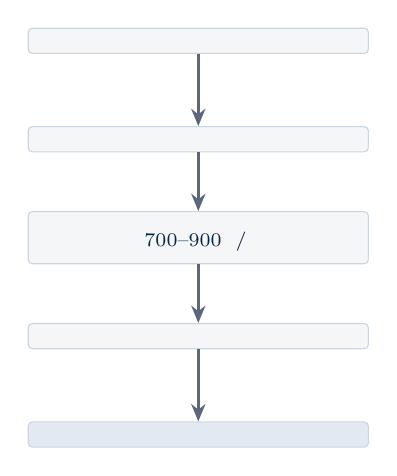
\begin{tikzpicture}[x=1cm,y=1cm]
  \node[chip,text width=4.0cm] (n1) at (0,0) {Солнце};
  \node[chip,text width=4.0cm] (n2) at (0,-1.25) {Открытые линии магнитного поля};
  \node[chip,text width=4.0cm] (n3) at (0,-2.50) {Быстрый солнечный ветер\\700--900\,км/с};
  \node[chip,text width=4.0cm] (n4) at (0,-3.75) {Магнитосфера};
  \node[chip,text width=4.0cm,fill=pale] (n5) at (0,-5.00) {Ионосфера};
  \foreach \a/\b in {n1/n2,n2/n3,n3/n4,n4/n5}
    \draw[arr] (\a) -- (\b);
\end{tikzpicture}
\end{column}
\begin{column}[T]{0.57\textwidth}
  \vspace{1mm}
  \begin{itemize}
    \item Корональные дыры --- области в солнечной короне с пониженной плотностью и t° плазмы
    \item Истекают самые быстрые потоки ветра
    \item До Земли ветер идёт 2--4 суток
    \item Оценка вклада площади КД на ионосферу
  \end{itemize}
  \vspace{2mm}
  {\footnotesize\color{muted}Если связь есть, она должна проявиться
   в ряду ПЭС со сдвигом на время переноса.}
\end{column}
\end{columns}
\end{frame}

% ---------------------------------------------------------------- 5
\begin{frame}[t]{Как регистрируют корональные дыры}
\begin{columns}[T,onlytextwidth]
\begin{column}[T]{0.46\textwidth}
  \fig[width=\linewidth]{coronal_hole.png}
  \source{Снимок: ИКИ РАН и ИСЗФ СО РАН.}
\end{column}
\begin{column}[T]{0.51\textwidth}
  {\footnotesize
  \begin{itemize}
    \item Канал EUV и мягкий рентген: SDO/AIA, SOHO/EIT, STEREO/EUVI
    \item Пониженные плотность и температура $\Rightarrow$ тёмные области
    \item Открытые линии поля $\Rightarrow$ быстрый солнечный ветер
    \item Дополнительно: магнитограммы SDO/HMI, радионаблюдения, коронографы
    \item Пороговая сегментация зависит от порога и условий наблюдений
  \end{itemize}}
\end{column}
\end{columns}
\end{frame}

% ---------------------------------------------------------------- 6
\begin{frame}[t]{GEC за 2025 год}
  \begin{center}
    \fig[height=3.85cm]{gec.png}
  \end{center}
  \vspace{0.5mm}
  \begin{columns}[T,onlytextwidth]
  \begin{column}[T]{0.49\textwidth}
    {\footnotesize
    \begin{itemize}
      \item SIMuRG: 15-минутный ряд, ~35 тыс. точек
      \item Максимум весной, минимум в июне--июле
    \end{itemize}}
  \end{column}
  \begin{column}[T]{0.49\textwidth}
    {\footnotesize
    \begin{itemize}
      \item Короткие всплески --- геомагнитные возмущения
    \end{itemize}}
  \end{column}
  \end{columns}
  \source{     Ряд GEC: SIMuRG, ИСЗФ СО РАН.}
\end{frame}

% ---------------------------------------------------------------- 7
\begin{frame}[t]{Радиоизображения СРГ}
\begin{columns}[T,onlytextwidth]
\begin{column}[T]{0.35\textwidth}
  \fig[width=\linewidth]{srh_3ghz.png}
  \source{Радиоизображение: СРГ, 3\,ГГц за 1 сентября 2026 02:30-03:30 UT}
\end{column}
\begin{column}[T]{0.62\textwidth}
  {\footnotesize
  \begin{itemize}
    \item Частота 3\,ГГц, Сибирский радиогелиограф
    \item Усреднение за час вокруг 03:00 и 07:00 UT
    \item 722 момента времени за 2025 год
    \item Яркостная температура в кельвинах
    \item Гелиопроекционная сетка на диске
  \end{itemize}}
\end{column}
\end{columns}
\end{frame}

% ---------------------------------------------------------------- 8
\begin{frame}[t]{Пороговая сегментация}
\begin{columns}[T,onlytextwidth]
\begin{column}[T]{0.33\textwidth}
  \fig[width=\linewidth]{srh_3ghz_processed.png}
  \source{После обработки: 0--100 тыс.\,К.}
\end{column}
\begin{column}[T]{0.64\textwidth}
  {\footnotesize
  \begin{itemize}
    \item Порог --- мода яркостной температуры всех пикселей
    \item Эта мода соответствует спокойному Солнцу
    \item Ниже порога --- области, похожие на КД
    \item Площадь --- в долях площади диска, безразмерная
    \item Результат чувствителен к порогу и условиям
  \end{itemize}}
\end{column}
\end{columns}
\end{frame}

% ---------------------------------------------------------------- 9
\begin{frame}[t]{Задержка солнечного ветра}
\begin{columns}[T,onlytextwidth]
\begin{column}[T]{0.44\textwidth}
  \begin{beamercolorbox}[wd=\linewidth,sep=3.5mm,rounded=true]{boxbg}
    {\color{muted}\footnotesize Время переноса для момента $t_i$}\par
    \vspace{1mm}
    {\large\color{navy}$\displaystyle \Delta t_i=\frac{R(t_i)}{v}$}\par
    \vspace{1mm}
    {\footnotesize\color{muted}$R(t_i)$ --- расстояние Солнце--Земля,
     $v$ --- скорость ветра}
  \end{beamercolorbox}
\end{column}
\begin{column}[T]{0.53\textwidth}
  {\footnotesize
  \begin{itemize}
    \item $R(t)$ --- по приближённой формуле орбиты
    \item Среднее $R=1.00037$\,а.е.
    \item $v=800$\,км/с --- скорость быстрых потоков
    \item Средняя задержка $\Delta t=2.165$\,сут
    \item GEC в $t_i+\Delta t_i$ --- линейная интерполяция
    \item Отброшены края и разрывы длиннее 24\,ч
  \end{itemize}}
\end{column}
\end{columns}

\vspace{2mm}
\begin{center}
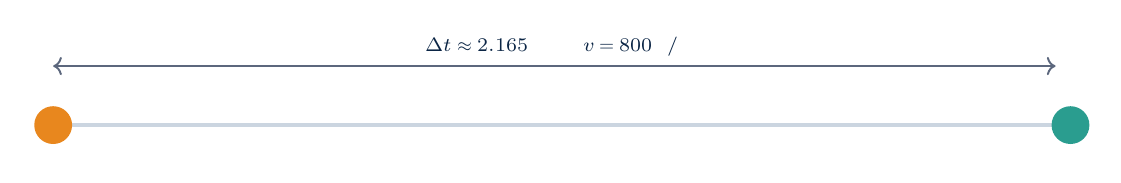
\begin{tikzpicture}[x=0.95cm,y=1cm]
  \draw[line width=1.6pt,edge] (0,0) -- (13.6,0);
  \fill[sun] (0,0) circle (2.4mm);
  \fill[teal] (13.6,0) circle (2.4mm);
  \node[below=1.4mm,font=\scriptsize,text=muted] at (0,0) {Солнце};
  \node[below=1.4mm,font=\scriptsize,text=muted] at (13.6,0) {Земля};
  \draw[<->,draw=muted,line width=0.7pt] (0,0.75) -- (13.4,0.75);
  \node[above,font=\scriptsize,text=navy] at (6.7,0.75)
    {$\Delta t\approx 2.165$ сут при $v=800$\,км/с};
\end{tikzpicture}
\end{center}
\end{frame}

% ---------------------------------------------------------------- 10
\begin{frame}[t]{Коэффициент корреляции}
\begin{columns}[T,onlytextwidth]
\begin{column}[T]{0.54\textwidth}
  \fig[width=\linewidth]{scatter_area_gec.png}
\end{column}
\begin{column}[T]{0.44\textwidth}
  \vspace{1mm}
  \bigresult{$r=-0.272$}\par\vspace{1.5mm}
  {\small $N=711$ пар;\quad $r^2=0.074$ --- около 7\,\% дисперсии}\par
  \vspace{3.5mm}
  {\scriptsize
  \renewcommand{\arraystretch}{1.3}
  \begin{tabular}{@{}ll@{}}
    \toprule
    Параметр & Значение \\
    \midrule
    Скорость $v$ & 800\,км/с \\
    Среднее $R$ & 1.00037\,а.е. \\
    Задержка $\Delta t$ & 2.165\,сут \\
    Число пар $N$ & 711 \\
    Коэффициент $r$ & $-0.272$ \\
    Детерминация $r^2$ & 0.074 \\
    \bottomrule
  \end{tabular}}
\end{column}
\end{columns}
\end{frame}

% ---------------------------------------------------------------- 11
\begin{frame}[t]{Как интерпретировать связь}
\begin{columns}[T,onlytextwidth]
\begin{column}[T]{0.485\textwidth}
  {\color{sun}\rule{\linewidth}{1.4pt}}\par\vspace{1.6mm}
  {\bfseries Вариант 1: физический}\par\vspace{0.8mm}
  {\footnotesize\color{muted}Площадь КД --- лишь один из источников
   вариаций GEC; её вклад теряется на общем фоне.}
\end{column}
\begin{column}[T]{0.485\textwidth}
  {\color{teal}\rule{\linewidth}{1.4pt}}\par\vspace{1.6mm}
  {\bfseries Вариант 2: методический}\par\vspace{0.8mm}
  {\footnotesize\color{muted}Пороговая сегментация неточно определяет
   реальную площадь корональных дыр.}
\end{column}
\end{columns}

\vspace{4mm}
{\small\key{Что говорит литература}}\par\vspace{1.2mm}
{\footnotesize
\begin{itemize}
  \item 9-дневные колебания термосферы --- вращающиеся КД
        (Fang et al., 2012)
  \item Субгармоники плотности ионосферы и скорости ветра
        (Tulasiram et al., 2010)
  \item Отклик на высокоскоростные потоки в отдельных событиях
        (Shimeis et al., 2012; Liu et al., 2019; Younas et al., 2022)
\end{itemize}}
\vspace{1mm}
{\scriptsize\color{muted}Но это событийный анализ или локализованный
 отклик, а не связь на годовом глобальном ряду.}
\end{frame}

% ---------------------------------------------------------------- 12
\begin{frame}[t]{Ограничения и что дальше}
\begin{columns}[T,onlytextwidth]
\begin{column}[T]{0.485\textwidth}
  {\color{muted}\rule{\linewidth}{1.4pt}}\par\vspace{1.6mm}
  {\bfseries Ограничения}\par\vspace{1mm}
  {\footnotesize
  \begin{itemize}
    \item Глобальное усреднение размывает широтные эффекты
    \item Одна скорость 800\,км/с на все события
    \item Два отсчёта в сутки --- грубая оценка задержки
    \item Нет положения КД на диске
    \item Нет данных за 26.11.2025
  \end{itemize}}
\end{column}
\begin{column}[T]{0.485\textwidth}
  {\color{sun}\rule{\linewidth}{1.4pt}}\par\vspace{1.6mm}
  {\bfseries Что дальше}\par\vspace{1mm}
  {\footnotesize
  \begin{itemize}
    \item ML-сегментация КД на радиоизображениях
    \item Положение и площадь КД на диске
    \item Скорость ветра для каждого события
  \end{itemize}}
  \vspace{2mm}
  {\scriptsize\color{muted}Площадь КД следует учитывать, но одной
   площади недостаточно.}
\end{column}
\end{columns}
\end{frame}

% ---------------------------------------------------------------- 13
{\setbeamertemplate{background canvas}{%
  
\begin{tikzpicture}[x=1cm,y=1cm]
    \useasboundingbox (0,0) rectangle (\paperwidth,\paperheight);
    \fill[navy] (0,0) rectangle (\paperwidth,\paperheight);
    \begin{scope}
      \clip (0,0) rectangle (\paperwidth,\paperheight);
      \foreach \r in {2.6,3.5,4.4,5.3,6.2} {
        \draw[sun,opacity=0.15,line width=0.6pt]
          ($(\paperwidth,0)+(2.0,2.4)$) circle[radius=\r];
      }
    \end{scope}
    \node[anchor=west,inner sep=0,align=left,text=white]
      at (2.0,0.5*\paperheight+0.4cm) {%
        \begin{minipage}{120mm}
          {\fontsize{46}{50}\selectfont\bfseries\color{sun}II}\\[1mm]
          {\color{sun}\rule{26mm}{1.8pt}}\\[5mm]
          {\fontsize{22}{27}\selectfont\bfseries Ионосфера и прогноз ПЭС}\\[5mm]
          {\small\color{lighttext}Площадь КД --- лишь один из входов.
           Чтобы проверить её вклад, нужен прогноз самой характеристики
           ионосферы.}
        \end{minipage}};
    \node[anchor=south east,inner sep=0,font=\scriptsize,text=lighttext]
      at (\paperwidth-1.0cm,0.7) {13\,/\,24};
  \end{tikzpicture}}
\begin{frame}[plain]\vspace*{0pt}\end{frame}}

% ---------------------------------------------------------------- 14
\begin{frame}[t]{TEC и GEC}
\begin{columns}[T,onlytextwidth]
\begin{column}[T]{0.44\textwidth}
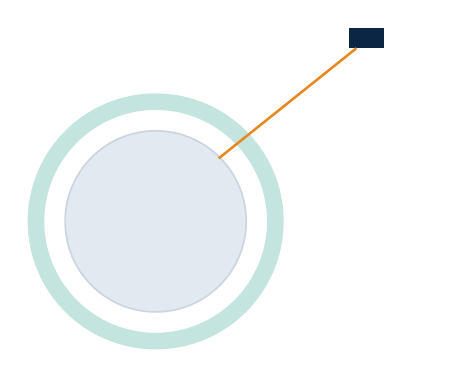
\begin{tikzpicture}[x=1cm,y=1cm]
  \fill[pale] (0,0) circle (1.15);
  \draw[edge,line width=0.6pt] (0,0) circle (1.15);
  \draw[teal,line width=6pt,opacity=0.28] (0,0) circle (1.52);
  \node[font=\scriptsize,text=muted] at (0,-0.10) {Земля};
  \node[font=\scriptsize,text=teal,anchor=west] at (1.60,-0.80) {ионосфера};
  \fill[navy] (2.45,2.20) rectangle ++(0.45,0.26);
  \node[font=\tiny,anchor=west,text=muted] at (2.95,2.33) {спутник};
  \draw[sun,line width=0.9pt] (2.55,2.20) -- (0.80,0.80);
  \node[font=\scriptsize,text=sun,anchor=south east] at (1.32,1.70) {луч};
\end{tikzpicture}
\end{column}
\begin{column}[T]{0.53\textwidth}
  \[
    TEC=\int N_e\,dl
  \]
  {\footnotesize
  \begin{itemize}
    \item 1\,TECU $=10^{16}$ электронов/м$^2$
    \item GEC --- глобальная характеристика ионосферы
    \item Зависит от EUV, геомагнитной активности, сезона и местного времени
    \item Применения: навигация, ВЧ-связь
  \end{itemize}}
\end{column}
\end{columns}
\end{frame}

% ---------------------------------------------------------------- 15
\begin{frame}[t]{Прогноз ПЭС: постановка задачи}
\begin{columns}[T,onlytextwidth]
\begin{column}[T]{0.48\textwidth}
  \fig[width=\linewidth]{ml_scheme.jpeg}
  \source{Схема: TecPredictionF10\_7.pptx.}
\end{column}
\begin{column}[T]{0.50\textwidth}
  {\footnotesize
  \begin{itemize}
    \item Эмпирических моделей много, но их входы обычно недоступны
    \item Цель: минимум входных данных и их история
    \item Прогноз глобальных карт ПЭС на разные горизонты
    \item Ключевой управляющий параметр --- индекс F10.7
    \item Дополнительно --- признаки даты и времени
  \end{itemize}}
  \vspace{1.5mm}
  {\scriptsize\color{muted}Между обучением и применением модель
   использует только F10.7 и календарь.}
\end{column}
\end{columns}
\end{frame}

% ---------------------------------------------------------------- 16
\begin{frame}[t]{Данные для прогноза}
\begin{columns}[T,onlytextwidth]
\begin{column}[T]{0.54\textwidth}
  {\scriptsize
  \renewcommand{\arraystretch}{1.45}
  \begin{tabular}{@{}ll@{}}
    \toprule
    Параметр & Значение \\
    \midrule
    Карты ПЭС & UQRG (UPC), 71$\times$72 \\
    Сетка & 5$^\circ$ по долготе $\times$ 2.5$^\circ$ по широте \\
    Индекс F10.7 & январь 1998 --- март 2024, шаг 1\,ч \\
    Обучение & 1998--2021 \\
    Валидация & 2022 \\
    Тест & 2023 --- март 2024 \\
    \bottomrule
  \end{tabular}}
\end{column}
\begin{column}[T]{0.44\textwidth}
  {\small\key{Признаки}}\par\vspace{1mm}
  {\footnotesize
  \begin{itemize}
    \item $\sin$ и $\cos$ циклов: 24\,ч, 27, 182.62, 365.25 и 4020 сут
    \item F10.7 на момент отсчёта
    \item F10.7 за 24\,ч до момента
    \item Среднее и медиана F10.7 за 27 и 180 сут
  \end{itemize}}
  \vspace{2mm}
  \[
    x_i=\sin\frac{2\pi t}{P_i},\qquad
    y_i=\cos\frac{2\pi t}{P_i}
  \]
\end{column}
\end{columns}
\end{frame}

% ---------------------------------------------------------------- 17
\begin{frame}[t]{Модель GIMini-LSTM-F10.7}
\begin{center}
  \fig[width=0.50\textwidth]{lstm_arch.jpeg}
\end{center}
\vspace{-1mm}
{\scriptsize\color{muted}
LSTM по истории F10.7 $\to$ 8 признаков; дата/время и F10.7
$\to$ 19 признаков; Dense(512)--Dropout--Dense(296) $\to$ Reshape $3\times1$;
два Conv2DTranspose $\to$ карта 71$\times$72.\par}
\vspace{1mm}
{\footnotesize Обучено и протестировано 70 моделей: 4 архитектуры,
 7 горизонтов (0--180 сут), три набора входных данных.}
\end{frame}

% ---------------------------------------------------------------- 18
\begin{frame}[t]{Пример прогноза}
\begin{columns}[T,onlytextwidth]
\begin{column}[T]{0.46\textwidth}
  \fig[height=0.70\textheight]{tec_forecast.jpeg}
\end{column}
\begin{column}[T]{0.52\textwidth}
  \vspace{2mm}
  {\small\key{GIMini-LSTM-F10.7-7}}\par\vspace{1.5mm}
  \begin{itemize}
    \item Прогноз на 2026-11-19, 01:00 UT
    \item Горизонт 7 суток, карта на конкретный час
    \item Шкала 0--90\,TECU, штриховая линия --- магнитный экватор
    \item Воспроизведены экваториальные гребни ПЭС
  \end{itemize}
  \vspace{2mm}
  {\footnotesize\color{muted}Детализация ограничена сеткой GIM
   5$^\circ\times$2.5$^\circ$.}
\end{column}
\end{columns}
\end{frame}

% ---------------------------------------------------------------- 19
\begin{frame}[t]{Сервис прогноза}
\begin{columns}[T,onlytextwidth]
\begin{column}[T]{0.47\textwidth}
  \fig[width=\linewidth]{forecast_ui.png}
\end{column}
\begin{column}[T]{0.47\textwidth}
  \vspace{2mm}
  {\footnotesize
  \begin{itemize}
    \item Выбор модели из списка доступных
    \item Календарь дат: 586 прогнозов в архиве
    \item Просмотр карты по часам, 0--23
    \item Выгрузка в \texttt{*.ionex} и \texttt{*.npz}
  \end{itemize}}
  \vspace{2mm}
  {\scriptsize\color{muted}Пример: GIMini-LSTM-F10.7-7,
   19 ноября 2026 г., 24 карты за сутки.}
\end{column}
\end{columns}
\end{frame}

% ---------------------------------------------------------------- 20
\begin{frame}[t]{Ограничения прогноза}
\begin{columns}[T,onlytextwidth]
\begin{column}[T]{0.56\textwidth}
  \fig[width=\linewidth]{rmse_table.png}
  \source{RMSE, TECU, по горизонтам прогноза.}
\end{column}
\begin{column}[T]{0.42\textwidth}
  \begin{itemize}
    \item RMSE растёт с горизонтом: 6.6\,TECU $\to$ 10.6\,TECU
    \item На сутки лучше IRI-2016 (11.08) и Klobuchar (15.00)
    \item Ошибки дают возмущения и разрешение GIM
    \item Развитие: учёт Kp и скорости ветра, ансамбли
  \end{itemize}
\end{column}
\end{columns}
\end{frame}

% ---------------------------------------------------------------- 21
\begin{frame}[t]{Два масштаба одной задачи}
\begin{columns}[T,onlytextwidth]
\begin{column}[T]{0.43\textwidth}
  \begin{beamercolorbox}[wd=\linewidth,sep=4mm,rounded=true]{}
    {\footnotesize\color{muted}Годовой ряд, глобальное усреднение}\\[1.5mm]
    {\bfseries Площадь КД $\rightarrow$ GEC}\\[2mm]
    {\large $r=-0.272$, $N=711$}\\[1mm]
    {\footnotesize\color{muted}слабая связь, $r^2\approx 0.074$}
  \end{beamercolorbox}
\end{column}
\begin{column}[T]{0.10\textwidth}
  \centering
  
\begin{tikzpicture}
    \draw[arr,line width=1.2pt] (0,0) -- (0.9,0);
  \end{tikzpicture}
\end{column}
\begin{column}[T]{0.43\textwidth}
  \begin{beamercolorbox}[wd=\linewidth,sep=4mm,rounded=true]{}
    {\footnotesize\color{muted}Карты на заданный час}\\[1.5mm]
    {\bfseries Прогноз карт TEC}\\[2mm]
    {\large RMSE $\approx 6.6$\,TECU}\\[1mm]
    {\footnotesize\color{muted}горизонт 1 сутки}
  \end{beamercolorbox}
\end{column}
\end{columns}

\vfill
\begin{center}

\begin{tikzpicture}
  \node[fill=sun,text=white,rounded corners=2pt,inner sep=3.2mm,
        font=\small,text width=13.2cm,align=center]
    {Данные СРГ \ + \ машинное обучение \ + \ ионосферные ряды\\[0.6mm]
     --- одна междисциплинарная задача};
\end{tikzpicture}
\end{center}
\end{frame}

% ---------------------------------------------------------------- 22
\begin{frame}[t]{Что мне может дать ШАД}
\vspace{7mm}

\begin{tikzpicture}[x=1cm,y=1cm]
  \node[card,anchor=north west,text width=4.1cm,minimum height=4.3cm] (a) at (0,0) {%
    {\color{sun}\bfseries\Large GPU}\\[1.5mm]
    {\bfseries Вычисления}\\[1.2mm]
    {\scriptsize\color{muted}Обучение моделей на больших рядах
     и глобальных картах TEC}};
  \node[card,anchor=north west,text width=4.1cm,minimum height=4.3cm] (b) at (4.7,0) {%
    {\color{sun}\bfseries\Large LLM}\\[1.5mm]
    {\bfseries Токены}\\[1.2mm]
    {\scriptsize\color{muted}Агентные пайплайны обработки данных
     и научных текстов}};
  \node[card,anchor=north west,text width=4.1cm,minimum height=4.3cm] (c) at (9.4,0) {%
    {\color{sun}\bfseries\Large ML}\\[1.5mm]
    {\bfseries Экспертиза}\\[1.2mm]
    {\scriptsize\color{muted}Нетворкинг и обратная связь
     по методам машинного обучения}};
\end{tikzpicture}
\end{frame}

% ---------------------------------------------------------------- 23
\begin{frame}[t]{Что я могу дать ШАД}
\vspace{7mm}
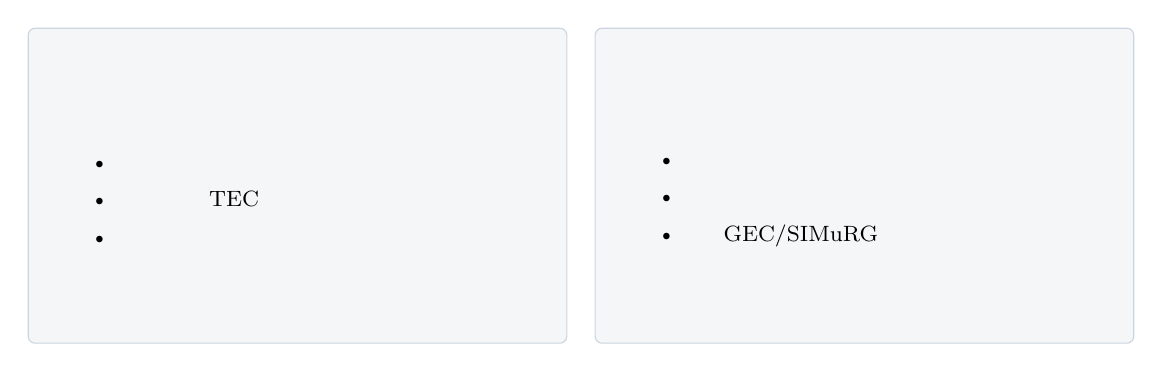
\begin{tikzpicture}[x=1cm,y=1cm]
  \node[card,anchor=north west,text width=6.2cm,minimum height=4.0cm] (a) at (0,0) {%
    {\color{teal}\bfseries\large Темы исследований}\\[2mm]
    {\footnotesize
     \begin{itemize}
       \item Сегментация корональных дыр
       \item Прогноз карт TEC
       \item Физически информированные модели
     \end{itemize}}};
  \node[card,anchor=north west,text width=6.2cm,minimum height=4.0cm] (b) at (7.2,0) {%
    {\color{teal}\bfseries\large Доступ к инструментам}\\[2mm]
    {\footnotesize
     \begin{itemize}
       \item Сибирский радиогелиограф
       \item Ионозонды ИСЗФ
       \item Ряды GEC/SIMuRG и архив изображений
     \end{itemize}}};
\end{tikzpicture}
\end{frame}

% ---------------------------------------------------------------- 24
{\setbeamertemplate{background canvas}{%
  
\begin{tikzpicture}[x=1cm,y=1cm]
    \useasboundingbox (0,0) rectangle (\paperwidth,\paperheight);
    \fill[navy] (0,0) rectangle (\paperwidth,\paperheight);
    \begin{scope}
      \clip (0,0) rectangle (\paperwidth,\paperheight);
      \foreach \r in {2.8,3.7,4.6,5.5,6.4,7.3} {
        \draw[sun,opacity=0.15,line width=0.6pt]
          ($(0,0)+(-1.6,1.2)$) circle[radius=\r];
      }
    \end{scope}
    \node[anchor=west,inner sep=0,align=left,text=white]
      at (2.0,0.5*\paperheight+1.0cm) {%
        \begin{minipage}{120mm}
          {\fontsize{30}{35}\selectfont\bfseries Спасибо за внимание}\\[3mm]
          {\color{sun}\rule{26mm}{1.8pt}}\\[6mm]
          {\normalsize Салимов Борис Гудратович}\\[1.5mm]
          {\small\color{lighttext}Институт солнечно-земной физики СО РАН}\\[1.5mm]
          {\small\color{lighttext}\texttt{salimov@iszf.irk.ru}}
        \end{minipage}};
    \node[anchor=south east,inner sep=0,font=\scriptsize,text=lighttext]
      at (\paperwidth-1.0cm,0.7) {24\,/\,24};
  \end{tikzpicture}}
\begin{frame}[plain]\vspace*{0pt}\end{frame}}

\end{document}
